\documentclass[a4paper]{article}    % define document layout
%\documentclass[draft]{article}     % use draft option in packages
%-----------------------------
% preamble
%-----------------------------
\usepackage[sumlimits,]{amsmath}    % math equations and formulas
\usepackage{amsfonts}
\usepackage[utf8]{inputenc}         % use UTF-8 encoding
\usepackage[english]{babel}         % use English language
\usepackage{graphicx}              % insert images
%\usepackage[draft]{graphicx}        % do not render figures
\usepackage{subcaption}             % multiple images in one figure
\usepackage{hyperref}               % hyperlinks
\usepackage{float}                  % floating objects (figures, tables)
\usepackage{geometry}               % page size and margins
\geometry{a4paper, margin=1in}      % margins
\usepackage{ragged2e}               % text alignment
\usepackage[table]{xcolor}          % change cell color in tables
%\usepackage{multirow}               % merge rows in table
%\usepackage[thinc]{esdiff}          % macros for derivatives
\usepackage{enumitem}

% MATLAB code
\usepackage{listings}
\usepackage{color} %red, green, blue, yellow, cyan, magenta, black, white
\usepackage{xcolor}

\graphicspath{                      % path for figures
    {../figures/} 
}

\definecolor{codegreen}{rgb}{0,0.6,0}
\definecolor{codegray}{rgb}{0.5,0.5,0.5}
\definecolor{codepurple}{rgb}{0.58,0,0.82}
\definecolor{backcolour}{rgb}{0.95,0.95,0.92}

\lstdefinestyle{mystyle}{
    backgroundcolor=\color{backcolour},   
    commentstyle=\color{codegreen},
    keywordstyle=\color{magenta},
    numberstyle=\tiny\color{codegray},
    stringstyle=\color{codepurple},
    basicstyle=\ttfamily\footnotesize,
    breakatwhitespace=false,         
    breaklines=true,                 
    captionpos=b,                    
    keepspaces=true,                 
    numbers=left,                    
    numbersep=5pt,                  
    showspaces=false,                
    showstringspaces=false,
    showtabs=false,                  
    tabsize=2
}
\lstset{style=mystyle}

%-----------------------------
% body
%-----------------------------
\begin{document}

\begin{figure}
    \centering
    % UNICAMP logo
    \begin{subfigure}{0.45\textwidth}
        \centering
        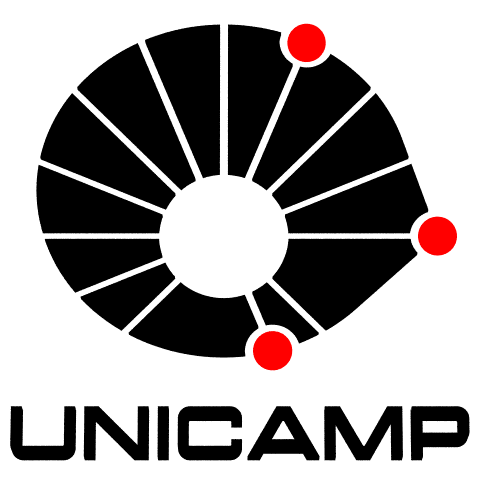
\includegraphics[width=1.5cm]{unicamp}
%        \label{fig:unicamp}
    \end{subfigure}
    \hfill
    % FEEC logo
    \begin{subfigure}{0.45\textwidth}
        \centering
        
\includegraphics[width=1.5cm]{feec}
%        \label{fig:feec}
    \end{subfigure}
\end{figure}

\title{
    \vspace{5cm}
    IA353A - Neural Networks\\
    EC2
    \vspace{1cm}
}
\author{
    Rafael Claro Ito\\
    (R.A.: 118430)
    \vspace{11cm}
}
%R.A.: 118430
%ito.rafael@gmail.com
\date{August 2020}
\maketitle
\newpage

\setcounter{section}{7}
%=================================================
\section*{Question 7}
%=================================================

%------------------------
\subsection{Transferência negativa}
%------------------------

%------------------------
\subsection{Camadas compartilhadas}
%------------------------

%------------------------
\subsection{MALSAR}
%------------------------

\newpage
%=================================================
\section*{Question 8}
%=================================================

\paragraph{Considerando a camada $q$ de uma rede neural, temos:}
\[x^{[q]} = f(W^{[q]} x^{[q-1]} + b)\]

\paragraph{Onde:}
\begin{itemize}
    \item $x^{[q]}$ é saída da camada $q$ após função de ativação;
    \item $W^{[q]}$ são os pesos dos neurônios da camada $q$;
    \item $x^{[q-1]}$ é a entrada camada $q$ (saída da camada $q-1$);
    \item $f(\cdot)$ é a função de ativação da camada $q$;
\end{itemize}

\paragraph{Calculando a variância de ambos lados da equação anterior, temos:}

\[x^{[q]} = f(W^{[q]} x^{[q-1]} + b)\]
\[Var(x^{[q]}) = Var(f(W^{[q]} x^{[q-1]} + b))\]

\paragraph{Devemos agora fazer algumas considerações:}
\begin{enumerate}[label=(\roman*)]
    \item função de ativação $f(\cdot) = tanh$, sendo que no início do treinamento trabalha-se com os pesos próximos à região linear (próximo de zero), evitando neurônios operando na região de saturação e favorecendo o aprendizado nas primeiras iterações. Desta forma, considerando a região linear, podemos aproximar a função $tanh$ para uma função identidade;
    \item $W$ e $x$ são independentes entre si;
    \item $W$ é uma variável aleatória i.i.d. (independente e identicamente distribuída). Isso geralmente é verdade para a inicialização.;
    \item $x$ é uma variável aleatória i.i.d. (independente e identicamente distribuída). Embora nem sempre isso seja verdade, por exemplo, pixels de uma imagem geralmente apresentam alta correlação entre pixels ao redor, faremos essa consideração;
\end{enumerate}

\paragraph{Continuando o desenvolvimento da equação anterior, temos:}
\[Var(x^{[q]}) = Var(f(W^{[q]} x^{[q-1]} + b))\]

\paragraph{A partir de i), temos:}
\[Var(x^{[q]}) = Var(W^{[q]} x^{[q-1]} + b)\]

\paragraph{Se duas variáveis são independentes entre si, temos a igualdade:\\
\href{https://en.wikipedia.org/wiki/Variance\#Product_of_independent_variables}{https://en.wikipedia.org/wiki/Variance\#Product\_of\_independent\_variables}:}
\[Var(XY) = [\mathbb{E}(X)]^2 Var(Y) + [\mathbb{E}(Y)]^2 Var(X) + Var(X)Var(Y)\]

\paragraph{Vamos agora abrir o produto das matrizes $W$ e $x$ em uma soma dos produtos de seus termos  $w_i$ e $x_i$. Usando também a consideração dada por ii) e sabendo que $b$ é uma constante (e portanto sua variância é zero), temos que:}
\[Var(x^{[q]}) = Var(W^{[q]} x^{[q-1]} + b)\]
\[Var(x^{[q]}) = Var(\sum_{i=1}^{n^{[q-1]}} w_i^{[q]} x_i^{[q-1]})\]
\[Var(x^{[q]}) = \sum_{i=1}^{n^{[q-1]}} Var(w_i^{[q]} x_i^{[q-1]})\]
\[Var(x^{[q]}) = \sum_{i=1}^{n^{[q-1]}}[\mathbb{E}(w_i^{[q]})]^2 Var(x_i^{[q-1]}) + [\mathbb{E}(x_i^{[q-1]})]^2 Var(w_i^{[q]}) + Var(w_i^{[q]})Var(x_i^{[q-1])}\]

\paragraph{A partir de iii) e iv), temos que $\mathbb{E}(w_i) = 0$ e $\mathbb{E}(x_i) = 0$. Sendo ambos $W$ e $x$ variáveis i.i.d. Assim:}
\[Var(x^{[q]}) = \sum_{i=1}^{n^{[q-1]}} Var(w_i^{[q]})Var(x_i^{[q-1]})\]
\[\boxed{Var(x^{[q]}) = n^{[q-1]} Var(w^{[q]})Var(x^{[q-1]})}\]

\paragraph{Queremos provar que $b = \sqrt{\frac{3}{n^{[q-1]}}}$ para que a variância da entrada da camada $q$ seja igual a variância da camada $q-1$.}

\paragraph{Sabendo que a variância de uma variável aleatória que segue uma distribuição uniforme entre $a$ e $b$, isto é, $X \sim \mathbb{U}[a,b]$, é dada por: $Var(X) = \frac{(b-a)^2}{12}$ (\href{https://proofwiki.org/wiki/Variance_of_Continuous_Uniform_Distribution}{prova}). Temos:}
\[Var(x^{[q]}) = n^{[q-1]} Var(w^{[q]})Var(x^{[q-1]})\]
\[Var(x^{[q]}) = n^{[q-1]} \cdot \frac{(b-(-b))^2}{12} \cdot Var(x^{[q-1]})\]
\[Var(x^{[q]}) = n^{[q-1]} \cdot \frac{(2b)^2}{12} \cdot Var(x^{[q-1]})\]
\[Var(x^{[q]}) = n^{[q-1]} \cdot \frac{4b^2}{12} \cdot Var(x^{[q-1]})\]

\paragraph{Como queremos $Var(x^{[q]}) = Var(x^{[q-1]})$, temos:}
\[n^{[q-1]} \cdot \frac{4b^2}{12} = 1\]
\[b^2 = \frac{12}{4 \cdot n^{[q-1]}}\]
\[\boxed{b = \sqrt{\frac{3}{n^{[q-1]}}}}\]

\newpage
\setcounter{section}{9}
\setcounter{subsection}{0}
%=================================================
\section*{Question 9}
%=================================================

%------------------------
\subsection{Principais seções do padrão de documentação}
%------------------------

%------------------------
\subsection{Artigos com propósitos similares}
%------------------------

%------------------------
\subsubsection*{Artigo 1}
%------------------------

%------------------------
\subsubsection*{Artigo 2}
%------------------------

\newpage
\setcounter{section}{10}
\setcounter{subsection}{0}
%=================================================
\section*{Question 10}
%=================================================

%------------------------
\subsection{EfficientNet}
%------------------------

%------------------------
\subsection{FixEfficientNet}
%------------------------

%=================================================

\end{document}
